
In industry, cranes are commonly used to lift heavy materials and transport them from location to location. In some cases, equipment or material may exceed the lifting capacity of a single crane or lifting fixture. In these cases, multiple cranes must be used to move the load. In order to ensure multi-crane lifts are performed safely, it must be ensured that each crane shares the load equally. Structural components known as equalizer beams are commonly employed to ensure that these loads are evenly distributed between the cranes. 


\begin{figure}
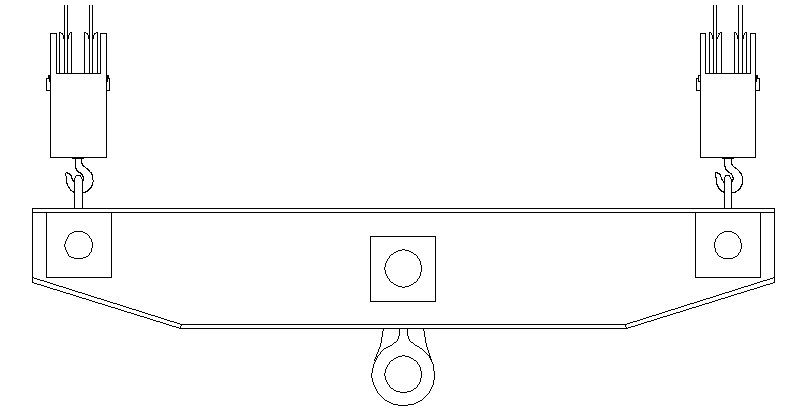
\includegraphics[width=\textwidth]{img/basic_eq_beam.png}
\label{img:basic_beam}
\caption{A Basic Equalizer Beam}
\end{figure}

Equalizer beams are typically single weldments with few, if any, moving parts. They are typically constructed from steel. The beam is typically built with 3 major attachment points. One for the load to be lifted, and 2 equidistant crane attachment points. The centers of the three attachment points are typically along the same axis to ensure equal load sharing between the two cranes, even in the event that the beam is out of level. A typical design for an equalizer beam is shown in Figure \ref{img:basic_beam}. 

Currently, the commonly accepted industry standard in use in the US is ASME BTH-1. This design standard lists recommended minimum design standards for these devices. This standard is widely accepted and is referenced in ASME's safety standard for below the hook devices, B30.20. The designs prepared and available for purchase in industry tend to be pre-engineered units utilizing standard components and beam sections. In some cases, the performance of these off-the-shelf components does not meet the needs of certain extremely stringent operating environments. Since the weight of rigging equipment is considered part of the lifted load, lifting heavy loads near the capacity of the cranes in use can require extremely weight-efficient rigging. At the same time, safety considerations require the stress in these components to be kept as low as achievable to maximize the margin of safety in the rigging system. Because these two objectives are often at odds with one another, design of these equalizer beams taking both objectives into account can be a difficult exercise for the designer. 

The nature of the competing requirements imposed against the design of equalizer beams makes them suitable for multiobjective optimization. In general, multiobjective optimization is intended to find a series of optimal solutions across a range of values for the two (or more) different design objectives and present them to a designer. For example, in the case of the equalizer beam, multiobjective optimization can present a series of optimal designs that have the lowest stress at numerous different weight values.  Using this technique, a designer can evaluate a number of designs at numerous different combinations of the design variables and select a design that best suits the situation. 


